\title{Changes on CRAN}
\subtitle{2021-01-01 to 2021-06-30}
\author{by Kurt Hornik, Uwe Ligges and Achim Zeileis}
\maketitle

\sloppy

\inputencoding{utf8}

In the past 6 months, 1290 new packages were added to the CRAN package
repository.  116 packages were unarchived and 467 were archived.  The
following shows the growth of the number of active packages in the CRAN
package repository:

\begin{figure}[h]
  \centering
  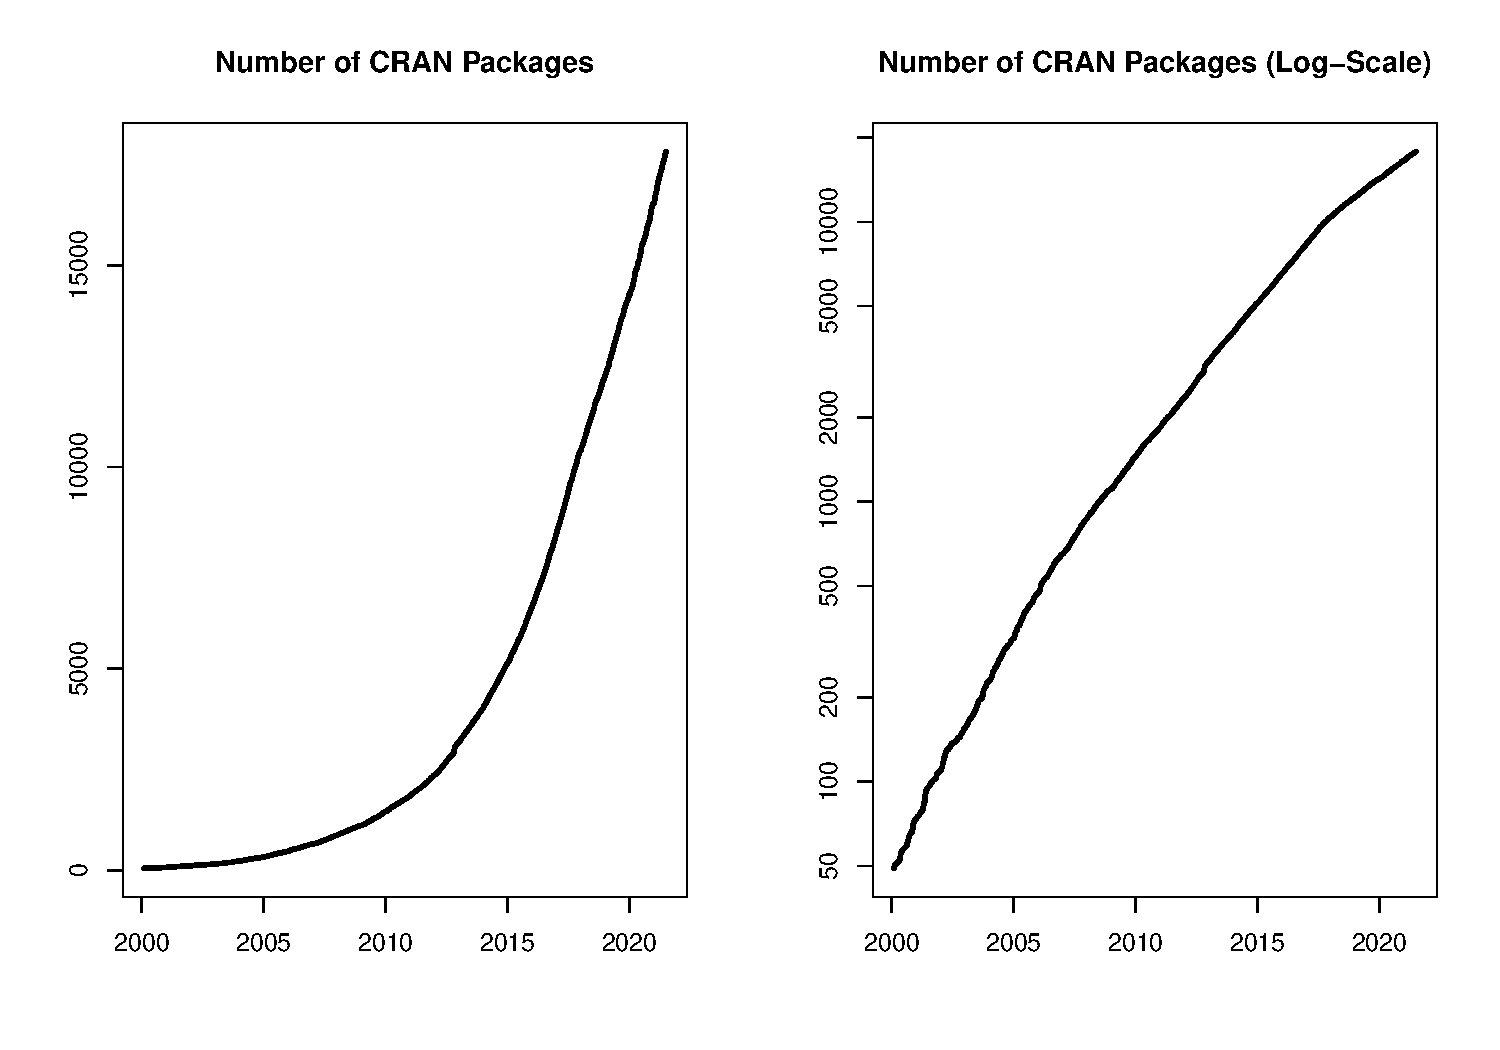
\includegraphics[width=5in]{cran_growth}
\end{figure}

\noindent
On 2021-06-30, the number of active packages was around 17778.




\subsection{CRAN package submissions}

During the the last three quarters (September 2020 to June 2021), CRAN received 25426
package submissions.
For these, 44844 actions took place of which 29039 (65\%) were auto
processed actions and
15805 (35\%) manual actions.

Minus some special cases, a summary of the auto-processed and manually
triggered actions follows:
\begin{center}
\begin{tabular}{l|rrrrrrrr}
       &  archive& inspect& newbies& pending& pretest& publish& recheck& waiting\\ \hline
auto  &   6191  &  5988 &  5585  &     0  &     0  &  7244  &  2429  & 1602  \\
manual&   6586  &    117&   874  &   855  &   249  &  5467  &  1322  & 335  \\
\end{tabular}
\end{center}

These include the final decisions for the submissions which were
\begin{center}
\begin{tabular}{l|rr}
action & archive        & publish\\ \hline
auto   &   5573 (22.5\%)  & 6131 (24.8\%)\\
manual &   6478 (26.2\%)  & 6544 (26.5\%)
\end{tabular}
\end{center}
where we only count those as \emph{auto} processed whose publication or
rejection
happened automatically in all steps.

%The CRAN team has changed. Martina Schmirl and Jelena Saf left the team.
%Thanks a lot to both of you!
%New members are Gregor Seyer who is very actively processing
%\emph{newbies} submissions and Julia Haider who just joined the team.
%Welcome to CRAN!

\subsection{CRAN mirror security}

%% ~/Work/R/CRAN_Admin/cran_secure_http_and_rsync.R

Currently, there are 103 official CRAN mirrors, 82 of which provide both
secure downloads via \samp{https} \emph{and} use secure mirroring from
the CRAN master (via rsync through ssh tunnels).  Since the R 3.4.0
release, \code{chooseCRANmirror()} offers these mirrors in preference to
the others which are not fully secured (yet).

\subsection{New packages in CRAN task views}

\begin{description}
    \item[\ctv{Bayesian}] \cpkg{causact}, \cpkg{dina}, \cpkg{edina},
        \cpkg{errum}, \cpkg{greta}, \cpkg{mcmcensemble}, \cpkg{rrum},
        \cpkg{shinybrms}.
    \item[\ctv{ClinicalTrials}] \cpkg{DTAT}, \cpkg{Keyboard},
        \cpkg{MinEDfind}, \cpkg{PowerUpR}, \cpkg{UnifiedDoseFinding},
        \cpkg{cosa}, \cpkg{crmPack}, \cpkg{presize}, \cpkg{randomizeR},
        \cpkg{replicateBE}, \cpkg{rpact}, \cpkg{simglm}.
    \item[\ctv{Cluster}] \cpkg{mdendro}, \cpkg{mixR}.
    \item[\ctv{DifferentialEquations}] \cpkg{RxODE}, \cpkg{mrgsolve},
        \cpkg{nlmixr}.
    \item[\ctv{Econometrics}] \cpkg{collapse}, \cpkg{ivreg}, \cpkg{lfe}.
    \item[\ctv{Finance}] \cpkg{AssetCorr}, \cpkg{LSMRealOptions},
        \cpkg{NFCP}, \cpkg{frenchdata}, \cpkg{garchmodels}.
    \item[\ctv{FunctionalData}] \cpkg{face}, \cpkg{mfaces},
        \cpkg{sparseFLMM}.
    \item[\ctv{HighPerformanceComputing}] \cpkg{proffer}, \cpkg{profile},
        \cpkg{profmem}, \cpkg{targets}.
    \item[\ctv{Hydrology}] \cpkg{AWAPer}, \cpkg{HydroMe},
        \cpkg{LWFBrook90R}, \cpkg{MODIStsp}, \cpkg{airGRdatassim},
        \cpkg{synthesis}, \cpkg{telemac}.
    \item[\ctv{MachineLearning}] \cpkg{DoubleML}, \cpkg{lightgbm}$^*$,
        \cpkg{mlpack}, \cpkg{splitTools}.
    \item[\ctv{MetaAnalysis}] \cpkg{CoTiMA}, \cpkg{DTAplots},
        \cpkg{EvidenceSynthesis}, \cpkg{MetaIntegration}, \cpkg{RoBMA},
        \cpkg{RobustBayesianCopas}, \cpkg{bnma}, \cpkg{boutliers},
        \cpkg{forplo}, \cpkg{fsn}, \cpkg{gmeta}, \cpkg{metaSurvival},
        \cpkg{metamicrobiomeR}, \cpkg{metapack}, \cpkg{nmaplateplot},
        \cpkg{smd}.
    \item[\ctv{MissingData}] \cpkg{InformativeCensoring}, \cpkg{NADIA},
        \cpkg{dejaVu}, \cpkg{grf}, \cpkg{idem}, \cpkg{lqr},
        \cpkg{misaem}, \cpkg{missRanger}, \cpkg{mixture}, \cpkg{norm2},
        \cpkg{samon}, \cpkg{semTools}.
    \item[\ctv{NumericalMathematics}] \cpkg{sanic}.
    \item[\ctv{OfficialStatistics}] \cpkg{collapse}, \cpkg{longCatEDA},
        \cpkg{sdcMicro}, \cpkg{simPop}.
    \item[\ctv{Optimization}] \cpkg{QPmin}, \cpkg{SPOT}, \cpkg{psqn},
        \cpkg{rminizinc}, \cpkg{rmoo}.
    \item[\ctv{Psychometrics}] \cpkg{ata}, \cpkg{tidyLPA}.
    \item[\ctv{ReproducibleResearch}] \cpkg{knitcitations},
        \cpkg{reportfactory}, \cpkg{targets}.
    \item[\ctv{Robust}] \cpkg{clubSandwich}, \cpkg{clusterSEs},
        \cpkg{skewlmm}.
    \item[\ctv{Spatial}] \cpkg{GWmodel}, \cpkg{RCzechia},
        \cpkg{chilemapas}, \cpkg{dbmss}, \cpkg{geobr}, \cpkg{geouy},
        \cpkg{giscoR}, \cpkg{ipdw}, \cpkg{mapSpain}, \cpkg{osmextract},
        \cpkg{rgee}, \cpkg{rgugik}, \cpkg{terra}.
    \item[\ctv{Survival}] \cpkg{Cyclops}, \cpkg{DAAG},
        \cpkg{InformativeCensoring}, \cpkg{LTRCtrees}, \cpkg{LogicReg},
        \cpkg{SGL}, \cpkg{SimSurvNMarker}, \cpkg{YPmodel},
        \cpkg{asbio}, \cpkg{bayesSurv}, \cpkg{bujar}, \cpkg{concreg},
        \cpkg{etm}, \cpkg{frailtyHL}, \cpkg{frailtySurv},
        \cpkg{frailtypack}, \cpkg{joineRML}, \cpkg{kmc}, \cpkg{kmi},
        \cpkg{mets}, \cpkg{mlr3proba}, \cpkg{npsurv}, \cpkg{plsRcox},
        \cpkg{reReg}, \cpkg{rstanarm}, \cpkg{simPH}, \cpkg{smoothSurv},
        \cpkg{spef}, \cpkg{superpc}, \cpkg{tranSurv}.
    \item[\ctv{TimeSeries}] \cpkg{HDTSA}, \cpkg{LSTS}, \cpkg{Rcatch22},
        \cpkg{Rsfar}, \cpkg{VARDetect}, \cpkg{autostsm},
        \cpkg{bayesforecast}, \cpkg{blocklength}, \cpkg{clock},
        \cpkg{collapse}, \cpkg{dynr}, \cpkg{fpcb}, \cpkg{gsignal},
        \cpkg{legion}, \cpkg{mfbvar}, \cpkg{strucchangeRcpp},
        \cpkg{tensorTS}, \cpkg{tsrobprep}.
    \item[\ctv{WebTechnologies}] \cpkg{AzureCosmosR}, \cpkg{AzureGraph},
        \cpkg{AzureKusto}, \cpkg{AzureQstor}, \cpkg{AzureTableStor},
        \cpkg{AzureVision}, \cpkg{Microsoft365R}.
\end{description}

(* = core package)

\address{Kurt Hornik \\
  WU Wirtschaftsuniversit\"at Wien, Austria \\
  \email{Kurt.Hornik@R-project.org}}

\address{Uwe Ligges \\
  TU Dortmund, Germany \\
  \email{Uwe.Ligges@R-project.org}}

\address{Achim Zeileis \\
  Universit\"at Innsbruck, Austria \\
  \email{Achim.Zeileis@R-project.org}}

